% PTE Core 模考 1B —— 口语 错题与详解·整理卷  版本 000（自包含）
% 编译: xelatex 本文件.tex   （需 Noto CJK + TeX Gyre Heros 字体）
% 本版本含图片，依赖同目录的 img/ 子目录。
\documentclass[11pt]{article}

% --------- 样式（原 ptestyle.sty，已内联）---------
% ============================================================
%  ptestyle.sty  —  PTE 模考错题整理卷 共享样式
%  编译引擎: XeLaTeX  (中英混排, 需要 Noto CJK 字体)
% ============================================================

\usepackage[a4paper,margin=2cm,headsep=4mm]{geometry}
\usepackage{fontspec}
\usepackage{xeCJK}
\usepackage[table]{xcolor}
\usepackage[normalem]{ulem}        % \sout 删除线
\usepackage{tabularx}
\usepackage{array}
\usepackage{ragged2e}
\usepackage{enumitem}
\usepackage[most]{tcolorbox}
\usepackage{fancyhdr}
\usepackage{graphicx}
\usepackage{needspace}
\usepackage{tikz}

% ---------- 字体 ----------
\setmainfont{TeX Gyre Heros}            % 拉丁: Helvetica 风格(纤细清晰)
\setCJKmainfont{Noto Sans CJK SC}
\setCJKsansfont{Noto Sans CJK SC}
\newfontfamily\cjkserif{Noto Serif CJK SC}
\linespread{1.18}
\setlength{\parindent}{0pt}
\setlength{\parskip}{4pt}

% ---------- 配色 ----------
\definecolor{cWrong}{HTML}{D32F2F}     % 红  = 修改 / 错误
\definecolor{cFix}{HTML}{1B7F3B}       % 绿  = 正确建议
\definecolor{cDelete}{HTML}{1565C0}    % 蓝  = 删除
\definecolor{cInsert}{HTML}{7B1FA2}    % 紫  = 插入
\definecolor{cPartial}{HTML}{E07B00}   % 橙  = 部分得分
\definecolor{cNote}{HTML}{0277BD}      % 蓝  = 注解
\definecolor{cAccent}{HTML}{16A085}    % 主题青绿(平台主色)
\definecolor{cWrongBg}{HTML}{FBE0E0}
\definecolor{cDelBg}{HTML}{DCE8FB}
\definecolor{cInsBg}{HTML}{EEE0F5}
\definecolor{cHead}{HTML}{20303A}
\definecolor{cGrayBox}{HTML}{F4F6F7}
\definecolor{cModelBg}{HTML}{EAF7EF}
\definecolor{cYouBg}{HTML}{FFF7F5}
\definecolor{cNoteBg}{HTML}{EAF3FA}
\definecolor{cRule}{HTML}{D7DEE2}

% ---------- 行内批改宏 (复刻平台标注) ----------
% \fix{原词}{正确}  红色删除线 + 绿色上标改正  (修改/拼写/空格)
\newcommand{\fix}[2]{%
  \colorbox{cWrongBg}{\textcolor{cWrong}{\sout{#1}}}%
  \,\textsuperscript{\textcolor{cFix}{\footnotesize #2}}}
% \del{原词}  蓝色删除线  (应删除)
\newcommand{\del}[1]{%
  \colorbox{cDelBg}{\textcolor{cDelete}{\sout{#1}}}%
  \,\textsuperscript{\textcolor{cDelete}{\footnotesize 删}}}
% \ins{词}  紫色下划线  (应插入)
\newcommand{\ins}[1]{%
  \textsuperscript{\textcolor{cInsert}{\footnotesize $\wedge$}}%
  \colorbox{cInsBg}{\textcolor{cInsert}{#1}}}
% \miss{词}  灰色删除线  (口语漏读 / 未作答)
\newcommand{\miss}[1]{\textcolor{gray}{\sout{#1}}}
% \add{原词}{改正}  橙色波浪线 + "补"标签  (平台漏标、本卷补标的错误)
\definecolor{cAdd}{HTML}{E65100}
\newcommand{\add}[2]{%
  \textcolor{cAdd}{\uwave{#1}}%
  \,\textsuperscript{\textcolor{cAdd}{\footnotesize 补：#2}}}
% 高亮(口语发音): 好/中/差
\newcommand{\spk}[2]{\textcolor{#1}{#2}}

% ---------- 评分单元格着色 ----------
\newcommand{\sfull}[1]{\textcolor{cFix}{\bfseries #1}}     % 满分
\newcommand{\spart}[1]{\textcolor{cPartial}{\bfseries #1}} % 部分
\newcommand{\szero}[1]{\textcolor{cWrong}{\bfseries #1}}   % 零/低分

% ---------- 分数小标签 ----------
\newtcbox{\chip}[1][cAccent]{on line, boxsep=2pt, left=4pt, right=4pt, top=1pt,
  bottom=1pt, arc=3pt, colback=#1, colframe=#1, coltext=white, nobeforeafter,
  fontupper=\bfseries\footnotesize}

% ---------- 题块小标题 ----------
\newcommand{\ptesub}[1]{%
  \par\needspace{2\baselineskip}\smallskip
  {\color{cAccent}\rule[-0.2ex]{3pt}{1.05em}}\hspace{6pt}%
  {\bfseries\color{cHead}#1}\par\nopagebreak\smallskip}

% ---------- 题块外框 ----------
% \begin{qblock}{标号·题型}{右上信息(得分/用时)} ... \end{qblock}
\newtcolorbox{qblock}[2]{
  breakable, enhanced, arc=2.5pt,
  colback=white, colframe=cRule, boxrule=0.6pt,
  left=11pt, right=11pt, top=8pt, bottom=10pt,
  toptitle=3pt, bottomtitle=3pt, lefttitle=11pt, righttitle=11pt,
  colbacktitle=cHead, coltitle=white, fonttitle=\bfseries,
  title={#1\hfill\normalfont\bfseries\small #2}}

% ---------- 文本块: 题干 / 范文 / 你的作答 / 建议 ----------
\newtcolorbox{promptbox}{enhanced, breakable, colback=cGrayBox, colframe=cGrayBox,
  arc=2pt, left=8pt, right=8pt, top=6pt, bottom=6pt, boxrule=0pt}
\newtcolorbox{modelbox}{enhanced, breakable, colback=cModelBg, colframe=cModelBg,
  borderline west={3pt}{0pt}{cFix}, arc=1pt, left=8pt, right=8pt, top=6pt, bottom=6pt, boxrule=0pt}
\newtcolorbox{youbox}{enhanced, breakable, colback=cYouBg, colframe=cYouBg,
  borderline west={3pt}{0pt}{cWrong}, arc=1pt, left=8pt, right=8pt, top=6pt, bottom=6pt, boxrule=0pt}
\newtcolorbox{notebox}{enhanced, breakable, colback=cNoteBg, colframe=cNoteBg,
  borderline west={3pt}{0pt}{cNote}, arc=1pt, left=8pt, right=8pt, top=6pt, bottom=6pt, boxrule=0pt}

% ---------- 评分表 ----------
% 用法见正文; 这里给表头宏
\newcommand{\scorehead}{%
  \rowcolors{2}{cGrayBox}{white}
  \arrayrulecolor{cRule}}

% ---------- 章节大标题 ----------
\newcommand{\ptesection}[3]{% #1=中文名 #2=英文名 #3=该项分数
  \needspace{6\baselineskip}
  \begin{tcolorbox}[enhanced, colback=cAccent, colframe=cAccent, sharp corners,
     left=14pt, right=14pt, top=10pt, bottom=10pt, boxrule=0pt]
    {\fontsize{20}{24}\selectfont\bfseries\color{white} #1\ \ }%
    {\large\color{white!85} #2}\hfill
    {\large\color{white}本项得分\ \ }{\fontsize{22}{24}\selectfont\bfseries\color{white} #3}%
    \ {\color{white!85}/ 90}
  \end{tcolorbox}}

% ---------- 题型小节分隔 (口语 RA/RS/DI/RTS/ASQ 等) ----------
\newcommand{\ptetask}[2]{%
  \needspace{4\baselineskip}\medskip
  \begin{tcolorbox}[enhanced, colback=cHead, colframe=cHead, sharp corners,
     left=12pt, right=12pt, top=5pt, bottom=5pt, boxrule=0pt]
    {\large\bfseries\color{white} #1}\ \ {\color{white!80} #2}
  \end{tcolorbox}\smallskip}

% ---------- 口语 AI 语音识别着色 (复刻平台: 优/良/差 + 停顿) ----------
\definecolor{cSpkGood}{HTML}{2E9E5B}   % 优 绿
\definecolor{cSpkOk}{HTML}{C77F00}     % 良 黄/琥珀
\definecolor{cSpkBad}{HTML}{E0352B}    % 差 红
\newcommand{\sg}[1]{\textcolor{cSpkGood}{#1}}   % 优
\newcommand{\sy}[1]{\textcolor{cSpkOk}{#1}}     % 良
\newcommand{\sr}[1]{\textcolor{cSpkBad}{#1}}    % 差
\newcommand{\smiss}[1]{\textcolor{cSpkBad}{\sout{#1}}}  % 漏读 (红删除线)
\newcommand{\pse}{{\color{gray}\,/\,}}          % 停顿
\newcommand{\asrlegend}{{\footnotesize\color{gray}AI 语音识别\quad
  {\color{cSpkGood}\textbullet}\,优\ \ {\color{cSpkOk}\textbullet}\,良\ \
  {\color{cSpkBad}\textbullet}\,差\ \ {\color{gray}/}\,停顿\ \
  {\color{cSpkBad}\sout{词}}\,漏读}}
\newtcolorbox{asrbox}{enhanced, breakable, colback=white, colframe=cRule,
  boxrule=0.6pt, arc=1pt, left=8pt, right=8pt, top=6pt, bottom=6pt}

% ---------- 颜色图例 ----------
\newcommand{\ptelegend}{%
  \begin{tcolorbox}[enhanced, colback=cGrayBox, colframe=cRule, boxrule=0.5pt,
    arc=2pt, left=10pt, right=10pt, top=6pt, bottom=6pt]
  {\bfseries\color{cHead}颜色说明\quad}
  \fix{改}{正}~修改/拼写\quad
  \del{删}~应删除\quad
  \ins{插}~应插入\quad
  \add{补}{改正}~平台漏标(本卷补标)\quad
  {\color{cFix}\rule{1em}{0.6em}}~范文/正确\quad
  {\color{cNote}\rule{1em}{0.6em}}~AI 建议
  \end{tcolorbox}}

% ---------- 页眉页脚 ----------
\pagestyle{fancy}
\fancyhf{}
\renewcommand{\headrulewidth}{0.4pt}
\renewcommand{\footrulewidth}{0pt}
\fancyhead[L]{\footnotesize\color{cHead}\bfseries PTE Core 模考 1B}
\fancyhead[R]{\footnotesize\color{gray} 错题与详解整理卷}
\fancyfoot[C]{\footnotesize\color{gray}\thepage}

\begin{document}

% --------- 封面（原 cover.tex）---------
% ---------- 封面 / 成绩总览 ----------
\definecolor{mListen}{HTML}{1F3A5F}
\definecolor{mRead}{HTML}{C2D70B}
\definecolor{mSpeak}{HTML}{4D4D4D}
\definecolor{mWrite}{HTML}{A01B7D}

\begin{titlepage}
\thispagestyle{empty}
\centering
\vspace*{1.4cm}

{\fontsize{30}{36}\selectfont\bfseries\color{cHead} PTE Core 模考 1B}\\[4mm]
{\fontsize{17}{20}\selectfont\color{cAccent}\bfseries 错题与详解 · 整理卷}\\[3mm]
{\color{gray} APEUni / 猩际 PTE 模考　·　提交时间 2026-06-21 12:36}\\[1.2cm]

% ---- 总分 ----
\begin{tcolorbox}[width=0.62\textwidth, halign=center, enhanced,
  colback=cAccent, colframe=cAccent, arc=6pt, boxrule=0pt, top=10pt, bottom=10pt]
  {\color{white}\large 总分 Overall}\\[2pt]
  {\fontsize{46}{50}\selectfont\bfseries\color{white} 40}
\end{tcolorbox}

\vspace{1.0cm}

% ---- 四项分数条形图 ----
\begin{tcolorbox}[width=0.84\textwidth, enhanced, colback=white, colframe=cRule,
  boxrule=0.8pt, arc=4pt, left=18pt, right=18pt, top=14pt, bottom=14pt]
\setlength{\tabcolsep}{6pt}\renewcommand{\arraystretch}{1.7}
\sffamily
\begin{tabular}{@{}r@{\hskip 8pt}l@{\hskip 10pt}l@{}}
 \bfseries Listening 听力 & {\color{mListen}\rule{3.67cm}{0.42cm}} & {\bfseries\large 33}\\
 \bfseries Reading 阅读   & {\color{mRead}\rule{4.67cm}{0.42cm}}   & {\bfseries\large 42}\\
 \bfseries Speaking 口语  & {\color{mSpeak}\rule{3.22cm}{0.42cm}}  & {\bfseries\large 29}\\
 \bfseries Writing 写作   & {\color{mWrite}\rule{6.33cm}{0.42cm}}  & {\bfseries\large 57}\\
\end{tabular}\\[2mm]
{\footnotesize\color{gray} 满分 90　|　刻度: 条长 = 得分 / 90}
\end{tcolorbox}

\vfill
\begin{flushleft}\small\color{gray}
\textbf{说明:}本卷由本次模考的题目与"详解"截图逐题誊写、重新排版而成,完整保留每道题的
\emph{题干 / 原文、范文、你的作答、逐项评分、彩色批改与 AI 中文建议}。\\
所有错误按平台标注用颜色标出(见下方图例)。原始"详解"PDF 不可复制、仅截图,本卷内容均为人工对照誊录,若与原图有出入以原图为准。
\end{flushleft}
\vspace{4mm}
\ptelegend
\end{titlepage}

% --------- 口语正文（原 sec_speaking_body.tex）---------
% ===================== 口语 Speaking =====================
\ptesection{口语}{Speaking · RA + RS + DI + RTS + ASQ}{29}

\vspace{1mm}
{\small\color{gray} 依据「口语详解1」逐题誊录，并复刻平台的 \textbf{AI 语音识别配色}：
{\color{cSpkGood}\textbf{绿=优}}、{\color{cSpkOk}\textbf{橙=良}}、{\color{cSpkBad}\textbf{红=差}}、{\color{gray}/=停顿}、
{\color{cSpkBad}\sout{红删除线}}=漏读/未读准。含 RA$\times$7、RS$\times$11、DI$\times$3、RTS$\times$3、ASQ$\times$1。
DI 附原图与平台范文，RTS 附情景与平台参考答案。}
\vspace{1mm}

\begin{notebox}
{\footnotesize \textbf{一句话诊断：}内容/恰当性多为中上，但\textbf{发音 Pronunciation}（多在 14$\sim$25/90）与
\textbf{流利度 Fluency}（多在 10$\sim$20/90）全面偏低，停顿与卡顿多、弱读不到位——这是口语仅 29 分的核心原因。}
\end{notebox}

% ============================================================
\ptetask{RA 朗读}{Read Aloud · 内容 Content / 5　发音 Pronunciation / 90　流利度 Fluency / 90}

\begin{notebox}
{\footnotesize\textbf{平台 AI 共性建议：}①朗读不够流畅，卡顿/迟疑较多；②弱读词（and / but / or / it / is / that）发音没弱化到位；
③单词发音过慢或拖音，建议读快一点；④读错的词偏多，重点纠正{\color{cSpkBad}标红}与{\color{cSpkOk}标橙}的词。下方彩色文本即平台对你朗读的逐词评测。}
\end{notebox}

\begin{qblock}{RA 1\quad \#608\ \ Summerhill School}{总分 \textcolor{cAccent}{\bfseries 12} / 90}
\asrlegend
\begin{asrbox}
\sg{Summerhill School} \sg{was regarded with considerable suspicion} \pse \sg{by the educational establishment} \sy{Lessons} \sy{were optional} \pse \sy{for} \sg{pupils at the school} \pse \sg{and the government} \sg{of the school} \pse \sg{was carried out by a School Council} \pse \sy{of which which all the} \pse \sy{pupils} \sg{and staff were members} \pse \sg{with} \pse \sg{everyone having equal voting rights}
\end{asrbox}
{\small 评分：内容 \sfull{5/5}\quad·\quad 发音 \spart{14/90}\quad·\quad 流利度 \szero{10/90}}
\end{qblock}

\begin{qblock}{RA 2\quad Statistical chances (universities)}{总分 \textcolor{cAccent}{\bfseries 18} / 90}
\asrlegend
\begin{asrbox}
\sg{The survey found that the} \pse \sg{the} \sr{statistical chances} \sg{of someone from} \pse \sy{a} \pse \sy{poor} \sg{background being} \sy{accepted at} \sg{one of the country's most respected universities} \pse \sy{are far} \sg{lower than those of} \sg{a student from} \pse \sg{a wealthy family This means that} \pse \sy{the} \pse \sy{inequalities in society} \sg{are likely to be passed down from} \pse \sg{one generation to the next}
\end{asrbox}
{\small 评分：内容 \sfull{5/5}\quad·\quad 发音 \spart{22/90}\quad·\quad 流利度 \szero{15/90}}
\end{qblock}

\begin{qblock}{RA 3\quad Language diversity}{总分 \textcolor{cAccent}{\bfseries 16} / 90}
\asrlegend
\begin{asrbox}
\sy{Despite a number of events in recent years} \pse \sg{devoted to language} \pse \sy{diversity} \pse \sg{language endangerment} \pse \sy{and multilingualism} \pse \sy{as such as} \pse \sy{the} \pse \sy{International Year of Languages} \pse \sg{public awareness of the issues is still remarkably limited} \sg{Only one in four of the} \sr{population} \sg{know that half the languages of the world} \pse \sy{are} \pse \sy{so seriously endangered} \pse \sg{that they are unlikely to survive} \pse \sy{the present century}
\end{asrbox}
{\small 评分：内容 \sfull{5/5}\quad·\quad 发音 \spart{20/90}\quad·\quad 流利度 \szero{11/90}}
\end{qblock}

\begin{qblock}{RA 4\quad European \& American orchestras}{总分 \textcolor{cAccent}{\bfseries 18} / 90}
\asrlegend
\begin{asrbox}
\sg{The advantage} \sg{of the great} \sy{European} \sy{and} \pse \sy{American orchestras} \sg{is that they were} \pse \sg{able to establish their} \sy{iconic} \pse \sg{status in an age when their identity could become} \pse \sr{entrenched} \pse \sy{there} \pse \sy{was} \pse \sy{less competition} \sg{and it} \sg{was} \pse \sg{easier to} \pse \sy{create} \pse \sy{a brand} \sg{Not only did they} \sg{have the best halls} \pse \sy{they} \sr{attracted} \sg{the best musicians who} \sg{tended to} \pse \sg{stay put}
\end{asrbox}
{\small 评分：内容 \sfull{5/5}\quad·\quad 发音 \spart{23/90}\quad·\quad 流利度 \szero{13/90}}
\end{qblock}

\begin{qblock}{RA 5\quad Loggerhead turtle}{总分 \textcolor{cAccent}{\bfseries 16} / 90}
\asrlegend
\begin{asrbox}
\sy{It s time for this young} \sy{loggerhead} \sg{turtle to go to work} \sg{We can} \sr{tether} \sg{turtles in these little} \sy{cloth harnesses} \pse \sy{put them into} \pse \sy{this} \pse \sy{tank and dull} \sg{swimming place University of} \sg{North Carolina biologist Ken Loman} \sg{studies} \sg{sea turtles that} \pse \sy{that are programed from} \pse \sg{birth for an} \sg{extraordinary journey Mother turtles} \pse \sy{buried the} \sg{eggs} \pse \sg{on the} \pse \sg{beach and then} \pse \sr{returned} \pse \sg{to} \pse \sg{the sea and the eggs hatch to} \sg{about 50 to 60 days later}
\end{asrbox}
{\small 评分：内容 \sfull{5/5}\quad·\quad 发音 \spart{22/90}\quad·\quad 流利度 \szero{10/90}}
\end{qblock}

\begin{qblock}{RA 6\quad Agricultural science}{总分 \textcolor{cAccent}{\bfseries 17} / 90}
\asrlegend
\begin{asrbox}
\sg{While} \sy{advances} \sg{in agricultural science have always been critical to} \sg{ensuring we help feed the world} \pse \sg{its impact and importance is even} \sy{greater now} \pse \sy{as population} \pse \sy{grows at} \sg{a rapid rate and the availability} \pse \sy{of arable land steadily} \pse \sg{declines Science and technology solutions are} \sy{essential} \pse \sg{to meeting growing demand for} \sy{food} \pse \sy{maintaining market competitiveness and adapting to land mitigating} \pse \sg{risks}
\end{asrbox}
{\small 评分：内容 \sfull{5/5}\quad·\quad 发音 \spart{21/90}\quad·\quad 流利度 \szero{12/90}}
\end{qblock}

\begin{qblock}{RA 7\quad Globalization}{总分 \textcolor{cAccent}{\bfseries 12} / 90}
\asrlegend
\begin{asrbox}
\sg{The benefits and} \sy{disadvantages of} \sg{globalization are} \pse \sy{the} \pse \sy{subject of ongoing debate} \sg{The downside to} \sg{globalization can be seen in the increased risk} \pse \sg{for the transmission of diseases Globalization has of} \pse \sy{course} \pse \sy{led to great good too Richer nations} \pse \sy{now can} \pse \sy{come to the aid of poorer} \pse \sg{nations in} \sy{crisis} \sg{Increasing diversity in many countries has meant} \pse \sy{more opportunity to learn about} \pse \sg{and celebrate other cultures}
\end{asrbox}
{\small 评分：内容 \sfull{5/5}\quad·\quad 发音 \spart{15/90}\quad·\quad 流利度 \szero{10/90}}
\end{qblock}

% ============================================================
\ptetask{RS 复述句子}{Repeat Sentence · 总分 / 90　内容 / 3　发音 / 90　流利度 / 90}

{\small\color{gray} 下方为平台逐词评测：{\color{cSpkGood}绿=优}、{\color{cSpkOk}橙=良}、{\color{cSpkBad}红=差}、{\color{cSpkBad}\sout{红删除线}=漏读/未读准}。
内容分低（如 0.2$\sim$0.8/3）即漏词/错词多。}\smallskip

\newcommand{\rsitem}[5]{%
  {\small\textbf{\##1}\quad 总分 \textcolor{cAccent}{\bfseries #2}/90 \quad
   {\footnotesize\color{gray}内容 #3/3 · 发音 #4 · 流利度 #5}}\par\nopagebreak\smallskip}

\rsitem{1428}{48}{2.2}{59}{59}
\begin{asrbox}\sg{today's} \smiss{lecture} \sg{is} \smiss{canceled} \sg{because the lecturer is} \smiss{ill}\end{asrbox}\smallskip

\rsitem{1430}{32}{1.5}{64}{54}
\begin{asrbox}\smiss{i am} \sg{available} \smiss{this thursday} \sg{afternoon}\end{asrbox}\smallskip

\rsitem{1449}{34}{1.6}{55}{61}
\begin{asrbox}\smiss{tuition} \sg{fees} \smiss{will} \sg{vary} \smiss{according to the field of} \sg{study}\end{asrbox}\smallskip

\rsitem{1431}{24}{1.2}{59}{49}
\begin{asrbox}\sy{newspapers} \smiss{around the country} \sg{are} \smiss{reporting the stories of the} \sg{president}\end{asrbox}\smallskip

\rsitem{1429}{10}{0.8}{37}{21}
\begin{asrbox}\sg{the} \sr{department} \smiss{determines whether or not the candidates pass}\end{asrbox}\smallskip

\rsitem{1487}{27}{1.7}{51}{37}
\begin{asrbox}\sr{a} \sg{very basic} \smiss{feature of computing} \sg{is} \smiss{counting} \sg{and} \smiss{calculating}\end{asrbox}\smallskip

\rsitem{1450}{35}{1.8}{52}{50}
\begin{asrbox}\sg{note} \smiss{that} \sg{the deadline} \sy{of} \sg{the} \smiss{submission of proposals} \sg{has} \smiss{been} \smiss{extended} \sg{for} \sr{a} \sg{week}\end{asrbox}\smallskip

\rsitem{1451}{28}{1.4}{47}{57}
\begin{asrbox}\sg{all students} \smiss{must return the books to} \sg{the} \smiss{college} \sg{library} \smiss{before} \smiss{the end of the} \sg{term}\end{asrbox}\smallskip

\rsitem{1448}{42}{1.9}{56}{64}
\begin{asrbox}\sg{the} \smiss{current labor} \sg{force is} \smiss{more} \sg{competitive} \smiss{than it has been} \sg{for} \sy{a} \sy{long} \sg{time}\end{asrbox}\smallskip

\rsitem{1432}{13}{0.6}{51}{61}
\begin{asrbox}\smiss{foods containing overabundant calories supply little} \sg{or} \smiss{no} \smiss{nutritional} \sg{value}\end{asrbox}\smallskip

\rsitem{1488}{10}{0.2}{48}{38}
\begin{asrbox}\sg{the} \smiss{contemporary literature works have been broadened and extended through interpretation}\end{asrbox}

% ============================================================
\ptetask{DI 描述图}{Describe Image · 内容 Content / 5　发音 / 90　流利度 / 90}

\begin{qblock}{DI 1\quad \#577\ \ Age Group（人口年龄/性别金字塔）}{总分 \textcolor{cAccent}{\bfseries 57} / 90}
\begin{center}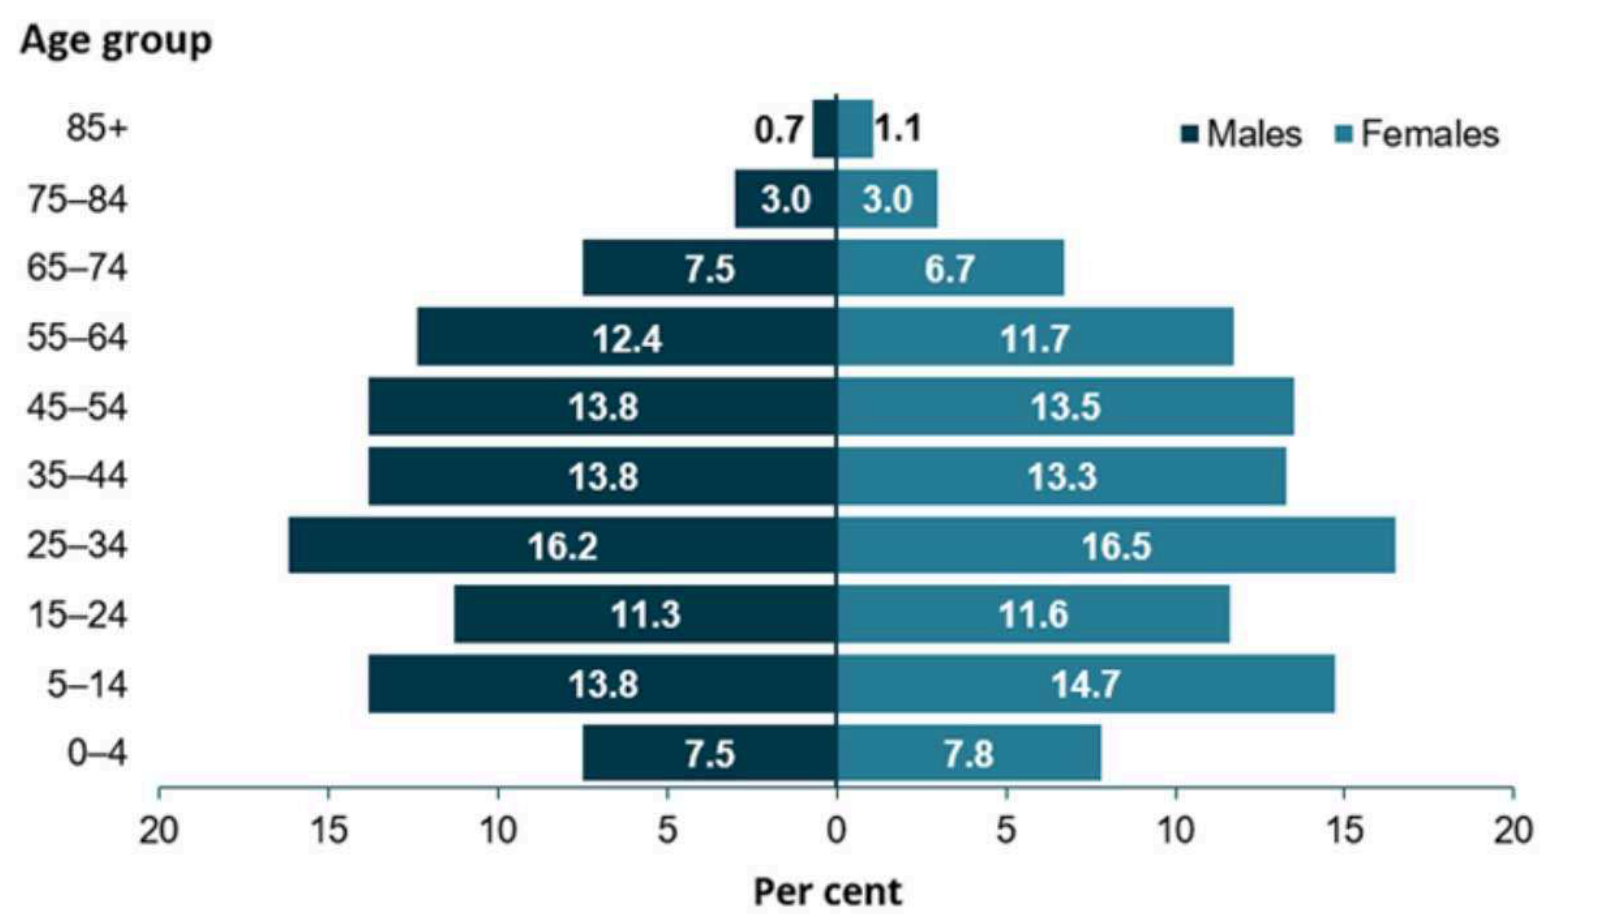
\includegraphics[width=0.95\linewidth]{img/di_age.png}\end{center}
\ptesub{范文 Model Answer（平台参考）}
\begin{modelbox}
The following graph gives information about percentages by age and sex. The items include age groups, female and male. According to this graph, in male, the value of eighty-five plus is around zero point seven, and that of seventy-five to eighty-four is higher, which is around three. You can see from this graph that the highest percentage of female is in twenty-five to thirty-four, above sixteen point five. What's more, the lowest share of male is zero point seven, for those above eighty-five. To sum up, the two areas have similar age distributions.
\end{modelbox}
\ptesub{你的作答 Your Response（AI 语音识别）}
\asrlegend
\begin{asrbox}
\sy{ok look at} \sg{these} \sy{pictures we can seize a x is present and} \sg{the} \sy{white is agent group and} \sg{as} \sy{below the left is may lands a right} \sy{is female} \sg{and} \sy{we can see that from twenty five to thirty four is} \sg{the} \sy{will} \sr{stir} \sy{a large people and} \sy{strewn t five} \sg{eight} \sy{choose a} \sy{thirty four for the females is the most part of them in like} \sy{eighteen five}
\end{asrbox}
{\small 评分：内容 \sfull{4.7/5}\quad·\quad 发音 \spart{71/90}\quad·\quad 流利度 \szero{33/90}}
\end{qblock}

\begin{qblock}{DI 2\quad \#567\ \ World Mobile Brands（澳洲手机品牌饼图）}{总分 \textcolor{cAccent}{\bfseries 55} / 90}
\begin{center}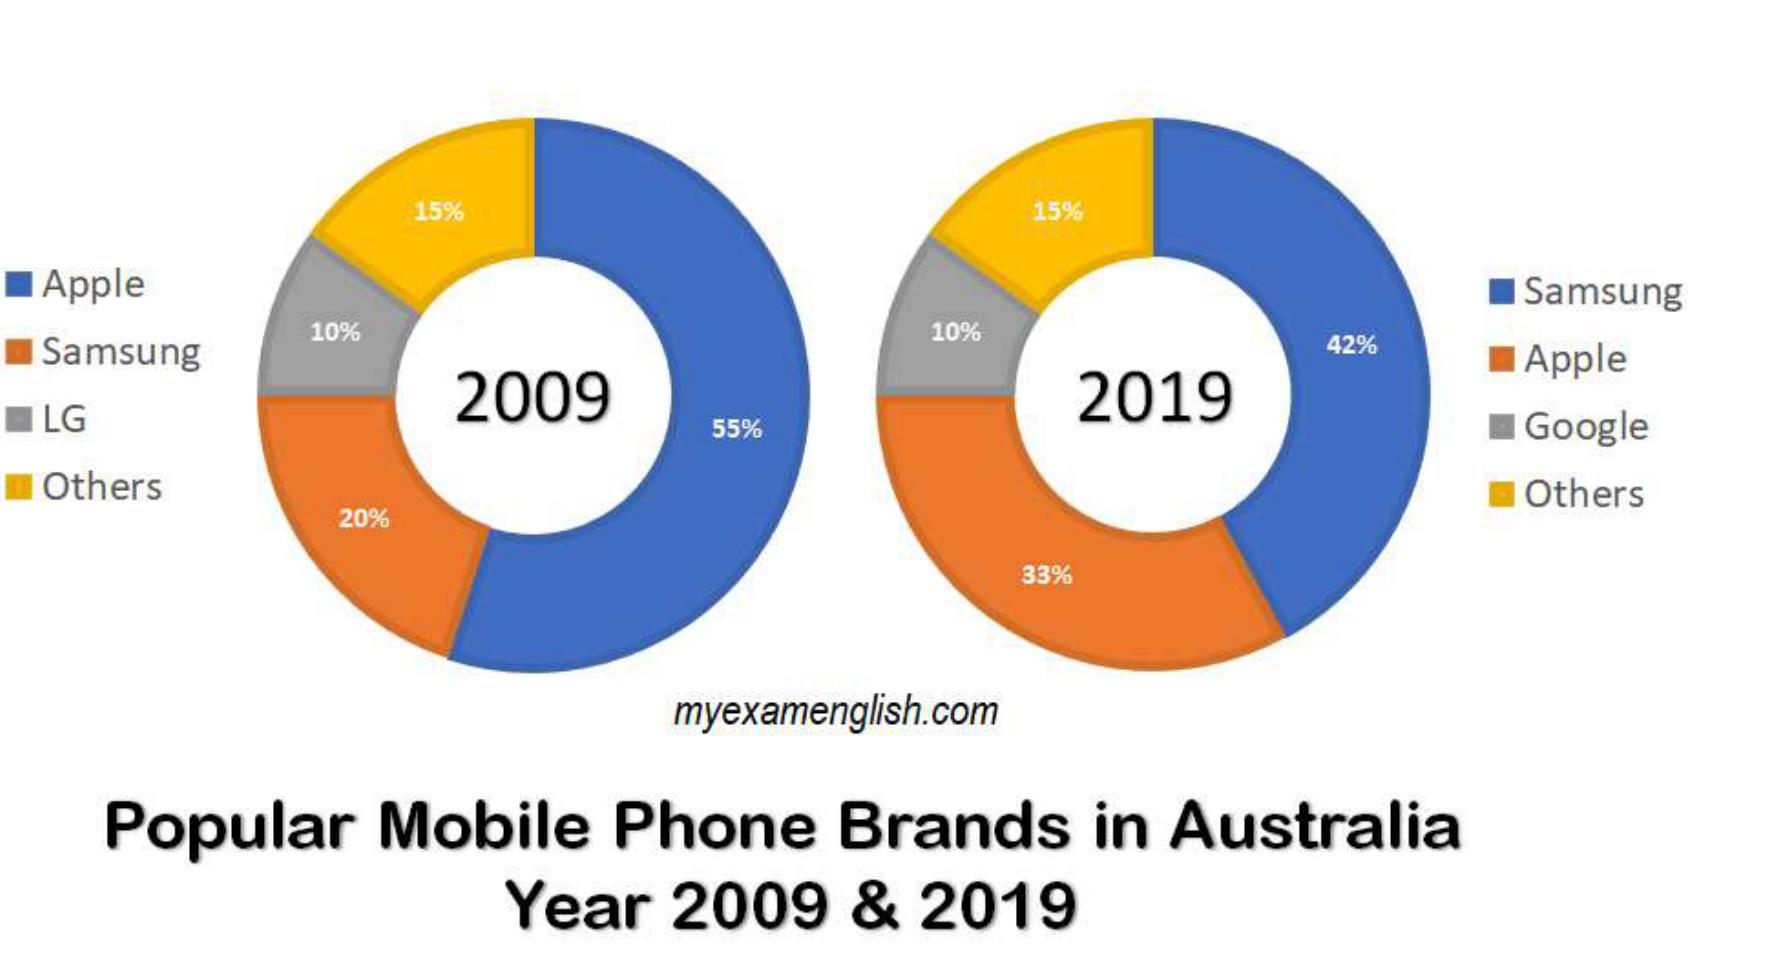
\includegraphics[width=0.86\linewidth]{img/di_phones.png}\end{center}
\ptesub{范文 Model Answer（平台参考）}
\begin{modelbox}
This pie chart gives information about popular mobile phone brands in Australia. From the chart we can see mobile phone brands include Apple, Samsung, LG and others. In two thousand and nine, Apple is the largest one, about fifty-five percent, followed by Samsung, about twenty percent. In twenty nineteen, Apple declines to thirty-three percent, and Samsung rises to forty-two percent. LG and others remain around ten percent and fifteen percent.
\end{modelbox}
\ptesub{你的作答 Your Response（AI 语音识别）}
\asrlegend
\begin{asrbox}
\sg{ok look} \sy{at} \sg{this} \sg{chart is about popular mobile phone brands in} \sg{australia year in nineteen nine and} \sy{nineteen nineteen and} \sy{twenty nineteen} \sr{a} \sg{we can see that ins} \sg{a left is about} \sy{twenty} \sg{and} \sg{nine is the most popular mobile phone brand is apple and from} \sg{the left} \sr{is} \sy{a twenty nineteen} \sg{the most popular} \sy{a} \sg{mobile phone} \sg{is still} \sy{is} \sy{essential} \sg{and} \sg{the next year april}
\end{asrbox}
{\small 评分：内容 \sfull{4.5/5}\quad·\quad 发音 \spart{73/90}\quad·\quad 流利度 \szero{35/90}}
\end{qblock}

\begin{qblock}{DI 3\quad \#576\ \ European Countries（欧洲地图）}{总分 \textcolor{cAccent}{\bfseries 48} / 90}
\begin{center}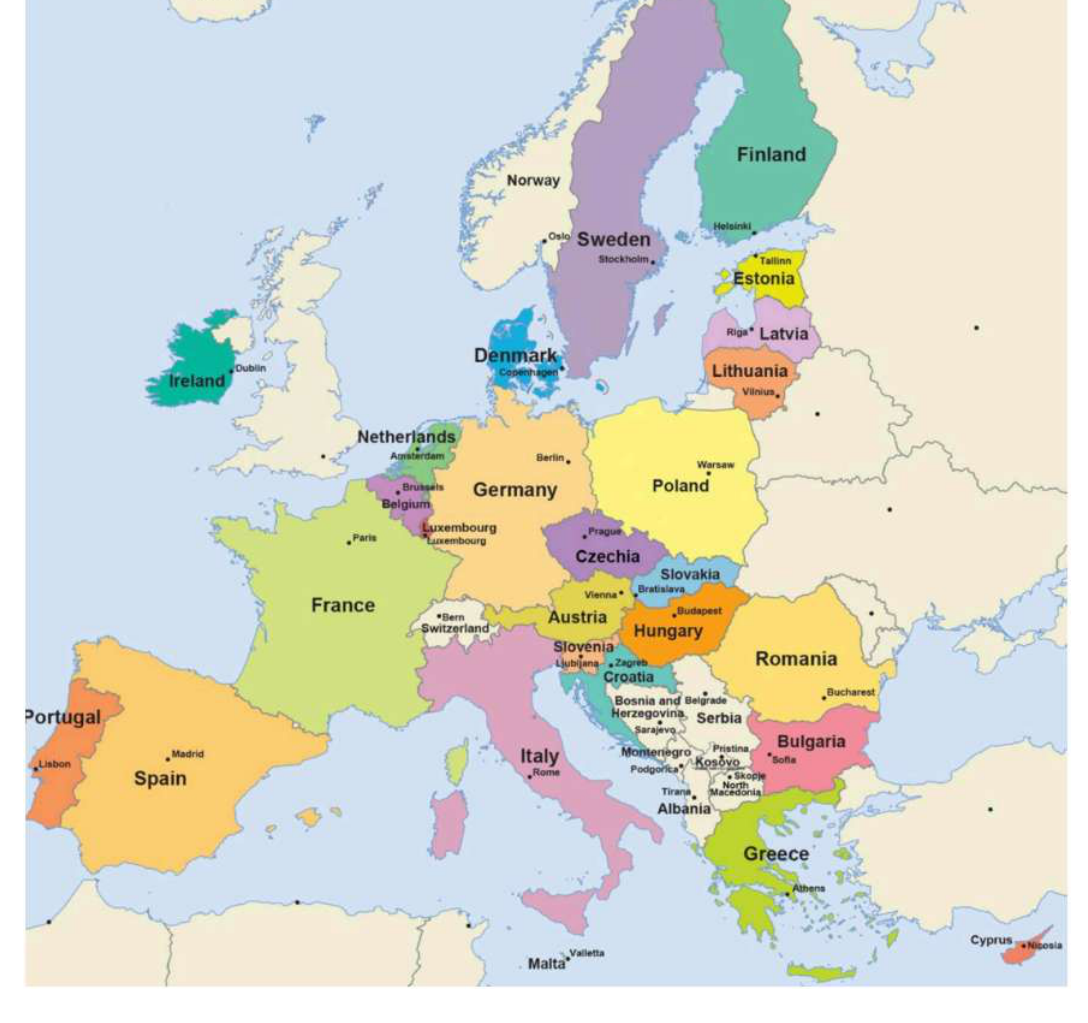
\includegraphics[width=0.52\linewidth]{img/di_map.png}\end{center}
\ptesub{范文 Model Answer（平台参考）}
\begin{modelbox}
The following graph gives information about Europe. Positions of different countries are displayed on the map. At the central area, we can see Austria, Germany, Poland and Czechia. In the left area, there lie Ireland and Portugal. According to this graph, the largest country is Russia, which is located on the right side. In comparison, small countries include Denmark and Belgium. In conclusion, there are many European countries shown on the map.
\end{modelbox}
\ptesub{你的作答 Your Response（AI 语音识别）}
\asrlegend
\begin{asrbox}
\sg{look at} \sg{this} \sy{image} \sg{a} \sg{we can} \sg{say it's a map} \sy{of} \sy{about european} \sy{a} \sg{like} \sy{australia and romania and g choose and we can see the} \sy{span is ins} \sg{a} \sr{deft} \sy{blows a maps and we can see is a} \sg{feel} \sy{and is a} \sy{ons um} \sy{a bit slow} \sg{and} \sy{a force of the map} \sg{and} \sy{the} \sy{germany and} \sg{australia is in} \sy{the} \sg{center of the map}
\end{asrbox}
{\small 评分：内容 \sfull{4.5/5}\quad·\quad 发音 \spart{64/90}\quad·\quad 流利度 \szero{28/90}}
\end{qblock}

% ============================================================
\ptetask{RTS 情景应答}{Respond to a Situation · 恰当性 Appropriateness / 90　发音 / 90　流利度 / 90}

\begin{qblock}{RTS 1\quad \#20\ \ Barbecue Party}{总分 \textcolor{cAccent}{\bfseries 24} / 90}
\ptesub{情景 Situation}
\begin{promptbox}
You've organized a barbecue with your friends at your place. However, upon their arrival, you notice some of your friends are using your kitchen utensils carelessly. You need to remind everyone to handle the utensils with care to maintain their quality and keep ourselves safe. What would you say to your friends?
\end{promptbox}
\ptesub{参考答案 Model Answer（平台参考）}
\begin{modelbox}
Hey everyone, thanks for coming over for the barbecue! Just a quick heads up, let's be careful with the kitchen utensils to avoid any accidents. I noticed some of them were getting a bit banged up. It's important to handle them with care to keep them in good shape and prevent any injuries. Let's enjoy the barbecue and make sure we clean up properly afterward. Thanks for understanding!
\end{modelbox}
\ptesub{你的作答 Your Response（AI 语音识别）}
\asrlegend
\begin{asrbox}
\sg{hi} \sr{i} \sg{notice that} \sr{some} \sg{of my friends are using} \sy{a} \sg{my kitchen} \sy{uses} \sy{careless i think i need to remind everyone to handles a} \sr{announces} \sg{with care} \sg{to maintain} \sy{your quality and} \sy{keep ourselves safe so i should say that you should handle your own} \sy{immunities to care about your own qualities and keep ourselves} \sy{safe}
\end{asrbox}
{\small 评分：恰当性 \spart{40/90}\quad·\quad 发音 \szero{21/90}\quad·\quad 流利度 \szero{19/90}}
\end{qblock}

\begin{qblock}{RTS 2\quad \#21\ \ Team-building Activity}{总分 \textcolor{cAccent}{\bfseries 19} / 90}
\ptesub{情景 Situation}
\begin{promptbox}
You've organized a team-building activity for your colleagues at a local park. However, upon arrival, you notice some team members are not participating actively and seem disengaged. You need to remind everyone of the importance of teamwork and encourage active participation to maximize the benefits of the activity. What would you say to your colleagues?
\end{promptbox}
\ptesub{参考答案 Model Answer（平台参考）}
\begin{modelbox}
Hey everyone, thanks for joining us for today's activity! Let's make sure we're all actively participating to get the most out of it. Remember, teamwork is key to our success, and by working together, we can achieve great things. Let's engage in the activities, share ideas, and support each other throughout. Together, we can strengthen our bond as a team and accomplish our goals more effectively. Let's dive in and make the most of this opportunity!
\end{modelbox}
\ptesub{你的作答 Your Response（AI 语音识别）}
\asrlegend
\begin{asrbox}
\sg{hi} \sr{i} \sg{think i have} \sy{noticed} \sg{that sound} \sr{him} \sg{members are not} \sy{participating activity and seems} \sy{disease} \sr{juice} \sg{i think} \sr{i} \sg{need to} \sg{remind everyone} \sy{of you} \sg{to} \sy{the importance of teamwork and} \sy{encourage active participant to} \sr{maximize} \sg{the benefit of} \sy{the t} \sg{so} \sy{i should i should say that every one} \sy{of our team should} \sg{know} \sr{the} \sy{importance} \sg{of} \sy{the} \sy{teamwork and you should be active um} \sg{be outgoing that's all}
\end{asrbox}
{\small 评分：恰当性 \spart{34/90}\quad·\quad 发音 \szero{14/90}\quad·\quad 流利度 \szero{15/90}\quad{\footnotesize\color{gray}（答题用时 01:30）}}
\end{qblock}

\begin{qblock}{RTS 3\quad \#22\ \ Community Garden Project}{总分 \textcolor{cAccent}{\bfseries 29} / 90}
\ptesub{情景 Situation}
\begin{promptbox}
You've organized a community garden project with your neighbors, and everyone's excited to start planting. However, upon arrival, you notice some garden beds are neglected, with weeds growing rampant. You need to remind everyone of their responsibility to maintain their assigned plots to ensure the success of the garden. What would you say to your neighbors?
\end{promptbox}
\ptesub{参考答案 Model Answer（平台参考）}
\begin{modelbox}
Hey everyone, thanks for being part of our project. But I noticed some of the garden beds are a bit neglected, with weeds taking over. Let's all remember our responsibility to maintain our assigned plots. Weeding regularly and keeping the beds tidy will help ensure the success of our garden. Together, we can create a beautiful and thriving green space for everyone to enjoy. Let's work together to keep our garden healthy and flourishing!
\end{modelbox}
\ptesub{你的作答 Your Response（AI 语音识别）}
\asrlegend
\begin{asrbox}
\sg{hi i have notice that some gardens fields} \sy{are} \sr{neglected} \sy{whiz} \sy{growing rapids i think i need to remind everyone of their} \sg{responsibility to} \sr{maintain} \sg{their} \sr{asylum} \sy{plots} \sg{to ensure the} \sg{success of the garden so i should say that} \sr{do} \sg{other things} \sy{to a} \sr{maintains era} \sy{science} \sr{abroad} \sg{to ensure the success of their} \sg{gardens}
\end{asrbox}
{\small 评分：恰当性 \spart{44/90}\quad·\quad 发音 \szero{25/90}\quad·\quad 流利度 \szero{24/90}}
\end{qblock}

% ============================================================
\ptetask{ASQ 简答}{Answer Short Question}

\begin{qblock}{ASQ\quad \#1189}{——}
\ptesub{问题 Question}
\begin{promptbox}
If someone tells you the truth, what is the opposite?
\end{promptbox}
\ptesub{参考答案 Answer}
\begin{modelbox}
Falsity\ /\ falseness\ /\ untruth
\end{modelbox}
{\footnotesize\color{gray} 你的作答：已录音（约 8 秒），截图未提供识别文字与单题得分。详解中仅含此 1 题 ASQ。}
\end{qblock}

\end{document}
